\documentclass[a4paper, 12pt, notitlepage]{article}
\usepackage{tikz}
\usetikzlibrary{shapes,arrows}
\usetikzlibrary{shapes.geometric}
\usepackage{fullpage}
\usepackage{wrapfig}
\usepackage{cite}
\usepackage{hyperref}
\usepackage{amsmath}
\usepackage{amsthm}
\usepackage{amssymb}
\usepackage{graphicx}
\usepackage{caption}
\usepackage{subcaption}

\author{Ryan Kinnear - 200273748 \\ Raza Rauf}
\title{FPGA Based Software Defined Radio Peripheral}
\date{\today}

\newtheorem{thm:NSST}{Nyquist-Shannon Sampling Theorem}

\begin{document}

\maketitle

\begin{abstract}
Wireless communication systems are a ubiquitous part of society and these systems, especially cellular systems, are advancing at an exponential rate.  Generally, significant portions of the communications protocols and algorithms (such as LTE) are implemented in monolithic integrated circuits.  This means that for a provider to update their system to a newer protocol, a lot of new hardware needs to be deployed - an expensive endeavor.  Implementing these algorithms in software enables wireless providers to upgrade to new protocols, add functionality, and fix problems simply by remotely downloading new code.  This approach is captured in the idea of software defined radio (SDR).  However, an SDR still requires a significant amount of electronics hardware (FPGAs, and analog ICs) between the antenna and the processor.  This hardware is known as the SDR peripheral.  The design and realization of an SDR peripheral is the objective of our project.  As a demonstration of functionality we will demodulate broadcast FM radio on an FPGA.
\end{abstract}

\newpage
\tableofcontents
\newpage
\listoffigures
\newpage

\section{Introduction}
\label{sec:intro}
Modern wireless systems are a ubiquitous part of society.  There are billions of people accessing the internet every day, many of them wirelessly.  This includes through home, office, or public WiFi networks, as well as through cellular networks.  The electromagnetic spectrum is also exploited for radio astronomy, Radio Frequency Identification (RFID), radar etc...  

In the past, all radio \footnote{The word \textit{radio} is used to refer to any device that makes use of the EM spectrum.  This does not refer only to communication systems, and certainly not only to radios made for receiving music} functionality was necessarily implemented in hardware using traditional electronics (transistors, capacitors, transformers...).  This also includes implementation with integrated circuits, even highly integrated devices with millions of transistors.  While the highly integrated ICs seem very modern, these radios offer no flexibility.  It is very costly to upgrade this type of radio equipment to take advantage of more modern protocols and algorithms - the entire device needs to be replaced.

The modern proliferation of high speed digital electronics, VLSI, and the mathematical understanding of digital signal processing has naturally lead to the integration of digital processing power and radio devices.  A lot of radio equipment uses digital signal processing to implement some of the signal chain.  However, this equipment is usually still highly integrated and static.

Reconfigurability and reprogrammability are big advantages.  A radio that has some dynamic reconfigurability is referred to as a \textit{software controlled radio}.  This may be a radio capable of dynamically choosing between the size of a QAM constellation based on noise levels, tuning the weights of a digital equalizing filter, or dynamically varying transmit power levels.  However, the fundamental demodulators are fixed in hardware and cannot be modified.  So the problem of upgrading radio equipment still exists to some extent.

Software defined radio (SDR) is a solution to the problem of limited flexibility.  In SDR, the vast majority of the signal processing is implemented in reconfigurable hardware (FPGAs \cite{fpga_defn}) or in software running on either a Digital Signal Processor (DSP \cite{dsp_defn}) or a General Purpose Processor (GPP) such as the one in your computer.  These devices are very easy to reconfigure, and thus the cost of upgrading to newer protocols and algorithms is drastically reduced.  Not only that but these upgrades or bug fixes can be performed remotely with ease.  Moreover, the ease with which the system is reconfigured allows one to use SDR as a test bed for development.

A further advantage of SDR is that both analog systems and integrated circuits are \textit{extremely} hard to design.  For a mixed signal integrated circuit that is 90\% digital, and 10\% analog, the analog design will take 90\% of the design time \cite{ana_why}.  Designing a new integrated circuit every time a new protocol needs to be implemented is \textit{extremely costly}.

%Write about how the report proceeds.
%Overview of SDR
%Our implementation
%Design goals and strategies
%Testing
%Uses of SDR
%Cognitive Radio

\subsection{git}
\label{sec:git}
The vast majority of the work from this project has been placed on github.  It can be found here: \url{https://www.github.com/RJTK/SDR_capstone}.  The files of interest will be the .spice (spice simulation) files and the .py files (Python).  These can be found in /model/ADC\_driver/ and /model/src/ respectively.  Many other files are either unimportant for the reader, or will be impossible to view correctly without the right software.   Specifically, the .pro, .sch, and .brd files are the files generated by the EDA tool KiCad \cite{kicad} that was used for schematic capture and PCB design.  The \LaTeX~ source for this report can be found in /docs/design\_reports/final\_report/.

\section{Fundamentals of SDR}
\label{sec:sdr_funadamentals}
\subsection{The Ideal SDR}
\label{sec:ideal_sdr}
An ideal SDR consists almost entirely of reconfigurable hardware and digital signal processing. The ultimate goal is to acheive flexibility and minimize the amount of analog design.  This ideal SDR would consist of an antenna, an analog to digital and digital to analog converter, a circulator, and a processor (see figure \ref{fig:ideal_sdr}).

%SDR architecture image
%------------------------------------------------------------------
%Damn this was hard to draw.

\tikzstyle{ADC} = [draw, fill=blue!20, text width=5em, 
    text centered, minimum height=2.5em]
\tikzstyle{DAC} = [draw, draw, fill=blue!20, text width=5em, 
    text centered, minimum height=2.5em]
\tikzstyle{Data} = [text width=5em, text centered, minimum height = 2.5em]
\tikzstyle{DSP} = [draw, text width=6em, fill=red!20, 
    minimum height=12em, rounded corners, text centered]
\tikzstyle{out} = [coordinate]
\tikzstyle{circulator} = [circle, draw, minimum height = 3em]
\tikzstyle{antenna} = [regular polygon, regular polygon sides = 3, thick, draw, fill=green!20, text width = 2em, shape border rotate = 180]

%\tikzstyle{antenna} = [draw]

\def\blockdist{2.3}
\def\edgedist{2.5}

\begin{figure}[ht]
\caption{Ideal SDR Architecture}
\label{fig:ideal_sdr}
\centering
\begin{tikzpicture}[auto, thick, node distance=2cm, >=latex']
  %The processor node goes right in the middle
  \node (processor) [DSP] {DSP / GPP};
  %Then place the ADC/DAC relative to the processor
  \path (processor.140)+(-\blockdist, 0) node (ADC) [ADC] {ADC};
  \path (processor.-140)+(-\blockdist, 0) node (DAC) [DAC] {DAC};
  %And draw arrows between them
  \draw [->] (ADC) -- (processor.west |- ADC);
  \draw [<-] (DAC) -- (processor.west |- DAC);
  
  %Place the circulator
  \path (processor)+(-3*\blockdist,0) node (circulator) [circulator] {CIRC};
  \draw [<-] (ADC.west) -- (circulator);
  \draw [->] (DAC.west) -- (circulator);

  \path (circulator)+(-1.2*\blockdist,0) node (antenna) [antenna] {ANT};
  \draw [<->] (antenna) -- (circulator.west);

  %Then place outputs relative to the processor
  \path (processor.150)+(2*\blockdist,0) node (out) [Data] {Data Out};
  \path (processor.-150)+(2*\blockdist,0) node (in) [Data] {Data In};
  %And arrows between them
  \draw [<-] (out) -- (processor.east |- out);
  \draw [->] (in) -- (processor.east |- in);

\end{tikzpicture}
\end{figure}
%------------------------------------------------------------------

This has the absolute minimum amount of analog components, and all of the signal processing is done in software.  While there is nothing wrong with this architecture in theory, it is obviously very difficult to implement in practice.  

Historically, the main problem was with the speed of the data converters.  However, there are now ADCs that can directly sample RF frequency signals \cite{gsps_adc}.  These ADCs are very sophisticated, and are far beyond the scope of this project.  We will see however that due to a concept called \textit{undersampling} \ref{sec:undersampling}.  This enables one to sample RF signals at rates far lower than twice the highest frequency component.

On the transmission side, it isn't possible to connect a DAC directly to an antenna.  There needs to be at least some analog components to provide power and filtering.

Another issue is the data rate.  A sample rate of 200MSPs is a torrent of data (1.5+ Gbps) and is beyond the capability of DSPs and GPPs.  This is where FPGAs and \textit{downsampling} (section \ref{sec:downsampling}) come in.  FPGAs are very effective for high speed data aquisition (DAQ) systems.

\subsection{Undersampling}
\label{sec:undersampling}
The Nyquist-Shannon Sampling Theorem is the most important theorem in digital signal processing.

\begin{thm:NSST}
\label{thm:NSST}
  If a function $f(t)$ is bandlimited to B hertz then $f(t)$ can be completely reconstructed from discrete samples of $f(t)$ at intervals $\frac{1}{2B}$.
\end{thm:NSST}

If we let $T = \frac{1}{2B}$ be the sampling interval, The specific formula for reconstruction is given by the sinc interpolator:

\begin{equation}
\label{eq:sinc_interpolation}
f(t) = \Big[\sum_{n=-\infty}^{\infty}{f(nT)\delta(t - nT)\Big]}*sinc(\frac{\pi t}{T}) = \sum_{n=-\infty}^{\infty}{f(nT)sinc(\pi\frac{t - nT}{T})}
\end{equation}

A critical piece of this theorem that seems to be frequently misunderstood is that the signal must be \textit{band limited} to B hertz.  This does \textit{not} mean that the highest frequency component needs to be below B hertz.  If the highest frequency component of the signal is below B hertz, then the assumptions of the theorem still hold.  It is a sufficient condition, however it is \textit{not necessary}.

If the signal is band limited to B hertz, but has spectral components greater than B (that is, it a band pass signal, see figure \ref{fig:bandpass_signal}), it is still possible to sample the signal without losing any information.  However, the effects of \textit{aliasing} will still be present.  But, aliasing is really not a big problem, as will be seen shortly.

\begin{figure}[ht]
\caption{A band pass signal with bandwidth B}
\label{fig:bandpass_signal}
\centering
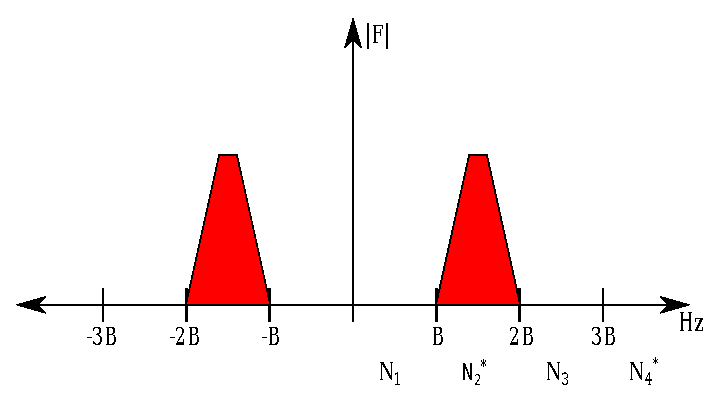
\includegraphics[width=11cm]{images/bandpass_signal.eps}
\end{figure}

The effect of sampling is to break up the frequency spectrum into ranges of width B.  That is, the frequency axis is partitioned into sets of the form $[nB, (n+1)B], n \in \mathbb{Z}$.  Each of these sets is referred to as a \textit{Nyquist Zone}.  They are labeled $N_1, N_2, ...$ in figure \ref{fig:bandpass_signal}.  Note that $N_1$ is the baseband.  Each of these zones will \textit{alias} or \textit{fold} back to baseband ($N_1$).  The best way to visualize this is to imagine folding the right half plane vertically at each $B, 2B, 3B ...$.  See figure \ref{fig:bandpass_sampling}.  Notice that the even nyquist zones get mirrored about the $B/2$ axis.

\begin{figure}[ht]
\caption{The effect of sampling}
\label{fig:bandpass_sampling}
\centering
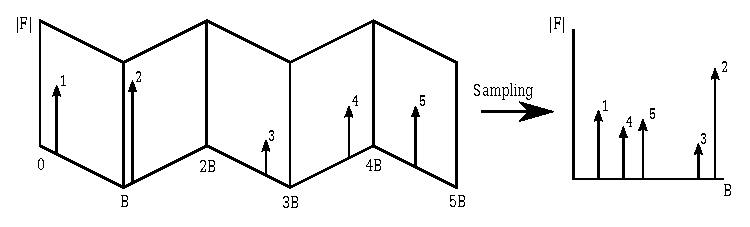
\includegraphics[width=13cm]{images/bandpass_sampling.eps}
\end{figure}

It should now be clear that analog to digital converters can be used to effectively digitize signals, even if they are at a very high frequency.  The only requirement is on the \textit{bandwidth} of the signal.  Naturally, a band pass filter is needed to cut out the out of band signals.  In undersampling a band pass filter is used for anti-aliasing. It seems to be commonly assumed that lowpass filters are always used for anti-aliasing, but this is only the case when sampling a signal in $N_1$.

There is another question to be looked at here, which is how to actually choose the sample rate?  If the spectrum of the signal you wish to digitize doesn't conveniently fall into one of the Nyquist zones, then some of the spectrum will be mirrored, and the other part won't be.  This will lead to a loss of information.  Also, it is convenient to ensure that the signal falls into an odd Nyquist zone, so that it doesn't get mirrored.  The criteria for the sampling rate can then be easily written down mathematically, where $f_c$ is the center frequency.

\begin{equation}
\label{eq:sample_rate}
\begin{aligned}
  &f_s > 2B \\
  &f_c - \frac{1}{2}B > nf_s \\
  &f_c + \frac{1}{2}B < \frac{1}{2}(2n + 1)f_s \\
\end{aligned}
\end{equation}

If for a given sample rate $f_s$, $\exists n \in \mathbb{N}$ satisfying the equations in (\ref{eq:sample_rate}) then that sample rate can be used to band pass sample the signal.  Moreover, $n+1$ gives the nyquist zone the signal falls into.

In practice, it is important to keep $n$ low.  There are practical problems associated with undersampling.  When the signal falls into a higher Nyquist zone the jitter on the ADC clock has a larger affect on the quality of the conversion.  The bandwidth of the input and any external components must also be high enough to pass the high frequency signal without adding too much distortion.

The ultimate reason that undersampling is often used in software defined radio is that it reduces the data rate to a level that digital hardware can deal with it.

\subsection{A Note on Oversampling}
%Oversampling doesn't actually help that much.
Why oversample when undersampling can do the job\cite{why_oversample}?  This is a good question.  There are some advantages of oversampling.  For example, if a signal is sampled $4n$ times it's bandwidth, and the samples are averaged \footnote{4 samples are averaged together to produce a single sample.  An example of downsampling, section \ref{sec:downsampling}}, the effective resolution of the conversion will be increased by $n$ bits \cite{oversample_extra_bits}.  So, to gain 1 extra bit of resolution (which would provide a theoretical maximum increase in SNR by about 6dB) the bit rate must increase by 400\%, 4 floating point operations need to be performed to produce 1 data sample (3 adds and a divide), the power consumption increases, and digital signal integrity issues get more complex.

The other main advantage of oversampling is that it can reduce the requirements on the anti-aliasing filter.  However in RF systems, a Surface Accoustic Wave (SAW) filter is often used for filtering, and these filters have extremely sharp cutoffs.

When sampling lower bandwidth signals, or when high quality filters are not available, the tradeoffs may be worth it.  For low bandwidth signals even if the sample rate is 20x higher than necessary, it still isnt ``high''.  But in the RF frequency domain, where sample rates already need to be quite high, the trade offs are usually not worth it.

\subsection{Downsampling and Multirate Signal Processing}
\label{sec:downsampling}
Changing the sample rate in a digital signal processing chain is a fundamental operation.  For example, CDs are recorded at 44.1KSPs but recording studios use much higher sample rates.  How do they change the sample rate from the studio recording to the sample rate required for CDs?  The answer is multirate digital signal processing \cite{multirate1} \cite{multirate2}.

To downsample a signal by a factor $M$, you simply throw away every $M^{th}$ sample (equation \ref{eq:downsampling}).  And, to upsample a signal by a factor $L$, you insert $L - 1$ 0's between every sample (equation \ref{eq:upsampling}).

\begin{equation}
\label{eq:downsampling}
y_D[n] = x[Mn] \qquad \text{Downsampling}
\end{equation}

\begin{equation}
\label{eq:upsampling}
y_U[n] = 
  \begin{cases}
    x[k] & \text{if } n = kL, k \in \mathbb{Z} \\
    0 & \text{otherwise}
  \end{cases}
  \qquad \text{Upsampling}
\end{equation}

By applying the properties of the Z-transform \cite{multirate2}, it can be shown that downsampling has the effect of ``compressing'' the frequency domain (equation \ref{eq:downsample_freq}), and upsampling has the effect of ``expanding'' it (equation \ref{eq:upsample_freq}).  Also remember that in the digital domain, there is an infinite number of copies of the spectrum placed at multiples of the sample rate.  These copies are still present in $X(\omega)$ and one needs to be very careful when visualizing equations \ref{eq:downsample_freq} \& \ref{eq:upsample_freq}.

\begin{equation}
\label{eq:downsample_freq}
Y_D(e^{j\omega}) = \frac{1}{M}\sum_{k=0}^{M-1}X(e^{j(\omega - 2\pi k)/M}) \qquad \text{Downsampling}
\end{equation}

\begin{equation}
\label{eq:upsample_freq}
Y_U(e^{j\omega}) = X(e^{j\omega L}) \qquad \text{Upsampling}
\end{equation}

Figure \ref{fig:multirate_freq} shows these effects visually in the frequency domaina.

\begin{figure}[ht]
\caption{Multirate in the Frequency Domain}
\label{fig:multirate_freq}
\centering
\includegraphics[width = 14cm]{images/multirate_freq.eps}
\end{figure}

Notice that downsampling causes aliasing.  In order to downsample, the signal first needs to be lowpass filtered to have a bandwidth less than $\frac{\pi}{M}$.  Likewise, when upsampling there are extra unwanted copies of the original signal that need to be filtered out.  For this reason, downsampling is usually preceeded by a lowpass filter, and upsampling is proceeded by a lowpass filter.

So, what is the point of downsampling?  The reason is that processing high speed digital data requires very fast hardware.  If the ADC is running at a modest 30MSPs with 12bits of width, then this is 360Mb/s.  And, if the entire signal processing chain requires a mere 20 operations per sample, then a processor capable of 600 million operations per second is required.  This isn't unobtainable, however it would definitely require a higher end device.  Most embedded processors run at rates well below 600MHz.  

Downsampling a signal can significantly reduce the data rate without losing any information.  This is the reason that FPGAs are so commonly used in software defined radio.  FPGAs are capable of massive parallelism and extremely high speeds.  FPGAs are ideal for implementing filters and up/down samplers (resampling) \footnote{resampling is the processes of either downsampling, upsampling, or a combination thereof.  Fractional resampling is achieved by cascading downsamplers and upsamplers.}.  After downsampling, the digital bitstream is passed on to the computer.

\subsection{Quadrature Demodulation}
\label{sec:quadrature_sampling}
A complex (as in complex numbers) representation of digital data is the last fundamentally important concept for SDR, and DSP in general.  A general sinusoid can be represented by the following formula \ref{eq:quadrature_sampling}.

\begin{equation}
\label{eq:quadrature_sampling}
A(t)cos(\omega t + \phi (t))
\end{equation}

Now, how can the phase $\phi(t)$ be discerned though regular samples of this signal?  And, how do you determine if $\omega$ is positive or negative?  Most importantly, how can these things be represented by discrete samples?  The answer is I/Q sampling.  The I stands for ``In phase'' and the Q stands for ``Quadrature''.  Formula \ref{eq:quadrature_sampling} can also be written as follows, by using some simple trigonometric identities.

\begin{equation}
\label{eq:trig_ident}
\begin{aligned}
  cos(\alpha)&cos(\beta) = \frac{1}{2}[cos(\alpha - \beta) + cos(\alpha + \beta)]\\
  sin(\alpha)&sin(\beta) = \frac{1}{2}[cos(\alpha - \beta) - cos(\alpha + \beta)]\\
\end{aligned}
\qquad \text{Product to Sum}
\end{equation}

It is then clear that

\begin{equation*} %* disables numbering
A(t)cos(\omega t + \phi (t)) = A(t)cos(\omega t)cos(\phi (t)) - 
A(t)sin(\omega t)sin(\phi(t))
\end{equation*}

Then we define

\begin{equation}
\label{eq:iq_defn}
\begin{aligned}
  &I(t) = A(t)cos(\phi (t))\\
  &Q(t) = -A(t)sin(\phi (t))\\
\end{aligned}
\end{equation}

to arrive at  

\begin{equation}
\label{eq:quadrature_sampling3}
A(t)cos(\omega t + \phi (t)) = I(t)cos(\omega t) + Q(t)sin(\omega t)
\end{equation}

To be clear, this gives us a way to represent the general sinusoid in equation \ref{eq:quadrature_sampling} by using a sum of a sine and a cosine.  To recover the original representation, simply apply the definitions of $I$ and $Q$.

\begin{equation}
\label{eq:quadrature_sampling4}
\begin{aligned}
A(t) &= \sqrt{I^2(t) + Q^2(t})\\
\phi(t) &= \tan^{-1}{\frac{Q(t)}{I(t)}}
\end{aligned}
\end{equation}

Finally, formula \ref{eq:quadrature_sampling4} can be interpreted geometrically (figure \ref{fig:quadrature_sampling}), and it becomes very convenient to use complex numbers to represent I/Q components.  That is, write the separate IQ components as a single complex number $I(t) + jQ(t)$.  This one complex number is a single IQ sample.

\begin{figure}[ht]
\caption{Geometric interpretation of formula \ref{eq:quadrature_sampling4}, and a complex number representation}
\label{fig:quadrature_sampling}
\centering
\includegraphics[width=8cm]{images/IQ_sample.eps}
\end{figure}

Since all of these quantities ($A, I, Q, \phi$) are time varying, they can be visualized as a helix in 3 dimensions.  This representation is far more enlightening than the typical 2D plots most of us are used to seeing.  For example, AM modulation can be seen with an IQ representation in figure \ref{fig:am_iq}, and PSK in figure \ref{fig:psk_iq}.

\begin{figure}
\begin{subfigure}[b]{0.45\textwidth}
  \centering
  \caption{AM} 
  \label{fig:am_iq}
  \includegraphics[width=\linewidth]{images/AM_IQ.png}
\end{subfigure}
\begin{subfigure}[b]{0.45\textwidth}
  \centering
  \caption{PSK}
  \label{fig:psk_iq}
  \includegraphics[width=\linewidth]{images/PSK_IQ.png}
\end{subfigure}

\caption{IQ Space Modulation}
\label{fig:iq_mod}
\end{figure}

The IQ representation is very powerful for digital processing because phase information is easily extracted.  The question remains, how to actually obtain the IQ samples?  The answer is by multiplying the signal separately by a cosine and a sine, both at the carrier frequency, then applying a low pass filter.

\begin{equation*}
\label{eq:quadrature_sampling5}
\begin{aligned}
  &A(t)cos(\omega t + \phi(t))cos(\omega t) = \frac{1}{2}A(t)cos(\phi(t)) + \frac{1}{2}A(t)cos(2\omega t + \phi (t))\\
  &A(t)cos(\omega t + \phi(t))sin(\omega t) = \frac{1}{2}A(t)sin(2\omega t + \phi(t)) - \frac{1}{2}A(t)sin(\phi(t))
\end{aligned}
\end{equation*}

Applying a lowpass filter (with a gain of 2) to these two quantities yields what should be recognized as the IQ components from equation \ref{eq:iq_defn}.

For a more general exposition of the effects of IQ demodulation in the frequency domain, see \cite{iq_sampling}.  However, our project is primarily related to demodulating FM broadcast radio and the preceeding information is enough.

\section{Project Overview and SDR Components}
SDR involves three main components.  An analog radio frequency front end \ref{sec:analog_frontend}, an FPGA (or other suitable high speed processing unit) \ref{sec:fpga}, and a software system \ref{sec:software}.  These three components and their relationship to our project are explained in this section.

\subsection{Analog Front End}
\label{sec:analog_frontend}
Any digital system that interfaces with the physical world necessarily involves some sort of analog component.  In radio systems, the analog front end (also referred to as the RF front end) involves everything between the antenna and the output of the analog to digital converter.  And, unlike the ideal architecture in \ref{sec:ideal_sdr} there is a significant amount of analog circuitry required.  It is necessary simply because the performance of analog to digital converters is a limiting factor.

The RF front end mixes down the analog RF signal to a rate more appropriate for analog to digital conversion.  It must also tune the system to select the correct frequency band.

The most popular radio architecture is the superheterodyne radio.  This system mixes down the RF frequency band to a common IF (intermediate frequency).  This means that regardless of which band the RF section is tuned to, it always mixes the band down to the same IF.  This radio architecture is very well suited to software radio applications because the IF frequency is fixed, there is no problem in picking a fixed sample rate.  This architecture can be seen in figure \ref{fig:superhet}

\begin{wrapfigure}{R}{0.55\textwidth}
  \centering
  \caption{Superheterodyne Radio Architecture}
  \label{fig:superhet}
  \includegraphics[width=.5\textwidth]{images/superhet.eps}
\end{wrapfigure}

%
% see /fourth_year/docs/app_notes/downconversion_architecture.pdf
% and write some more stuff about other architectures.
%

\subsection{FPGA}
\label{sec:fpga}
FPGAs are well suited for software defined radio for a variety of reasons.  One of the main reasons is that they are reconfigurable.  As explained in section \ref{sec:intro}, flexibility is essentially the whole point of SDR.  FPGAs are typically used to implement portions of the signal processing chain that require the fastest processing.  For example, FFTs, filters, channel selection, resampling, quadrature sampling etc...

The reason that FPGAs are necessary in the first place is that even after the signal is mixed down to a lower IF frequency, the required sample rate is still very high.  In our project in particular, the sample rate is 29MSPs.  Processing even this modest speed is beyond the capability of DSPs or GPPs.  The FPGA is suitable for high data rate computations that involve simple and fast operations, whereas general purpose processors are more suitable for algorithms that require a lot of decision making or intelligence.

\subsection{Software}
\label{sec:software}
The software in ``Software Defined Radio'', is obviously a quite substantial component.  Serious SDR packages such as GNURadio will contain on the order of hundreds of thousands of lines of code.  This software is quite generic, and can be used to process any digital data regardless of it's origin.  That is to say, we could potentially interface our hardware with a well developed SDR platform.  For research and development purposes it isn't necessary to develop custom software.  However, a commercial implementation would probably have custom code that is optimized for a particular platform or purpose.

Even though the signal processing software is very generic, that doesn't mean you can just plug any radio peripheral into your computer and expect it to work.  There needs to be a small layer of software between the SDR platform and the hardware peripheral, and this layer - called a \textit{driver} - needs to be unique to each hardware peripheral (and each operating system). \footnote{unless the hardware is explicitly designed to take advantage of existing drivers}.  This driver software operates in kernel space, and provides a generic interface between userspace code where the SDR software exists, and the SDR hardware.

\subsection{Project Scope}
The goals of our project are to implement an SDR \textit{peripheral}.  The peripheral is the hardware component that digitizes the RF waveform and after suitable preprocessing, sends the data to a computer.  We have went through a degree in electronics engineering, and thus we wish to focus on the hardware design.  Writing a driver to interface with our hardware, while still in the scope of work for an electrical engineer, is beyond the scope of our project.  The reason is that writing such a driver would be a substantial undertaking (for a non expert).  If our group was made up of 3 individuals rather than 2, an appropriate task for them would be to figure out how to interface our peripheral with GNURadio.

In order to incorporate a driver to interface in real time to an SDR platform like GNURadio would involve a large amount of work.  The person writing this driver would need to work closely with the FPGA developer in order to establish a communications protocol between the FPGA and the driver.  Then, they would need to write a module in GNURadio that interfaces with the driver.  Also consider that this driver needs to exist in kernel space.  Writing kernel space code is very different from writing user space code and would require a lot of background studying before even getting started.  For these reasons, we are keeping our computer interface as simple as possible.

%
% What computer interface did we use in the end.  Write stuff here.
%

\section{FM Demodulation Methods}
Our project is ultimately about building an SDR peripheral.  However, we also need some sort of demonstration of the system.  To this end, we will receive and demodulate a broadcast FM signal.

A Frequency Modulated (FM) signal can be represented using the form from equation \ref{eq:quadrature_sampling}.

\begin{equation}
  \psi_{FM}(t) = A(t)cos(2\pi f_c t + \int_{-\infty}^{t}m(\tau)d\tau)
\end{equation}

Where $m(t)$ is the analog message signal (the baseband).  When it is transmitted the amplitude of an FM modulated signal $A(t)$ is constant.  However, receivers cannot assume amplitude is constant because the channel will cause various distorting effects.

Intuitively, FM encodes information into the instantaneous frequency of the carrier signal.  An example of a simple FM signal can be seen in figure \ref{fig:fm_modulated_signal}.  An IQ space plot of an FM signal is not really any more insightful than just the regular 2D plot everyone is used to.

\begin{figure}
  \centering
  \caption{Example FM Modulation}
  \label{fig:fm_modulated_signal}
  \includegraphics[width=.7\textwidth]{images/fm_modulated_signal.png}
\end{figure}

There are various methods for demodulating an FM modulated signal.  Note however that FM is \textit{non-linear} modulation, it cannot be written simply as an s-domain transfer function, and the spectrum for a general FM signal cannot easily be written down.  It thus requires some non-linear components for demodulating it.  A few methods we considered are discussed below.  The demodulation scheme we chose is IQ demodulation, and it will be discussed in detail.

In essence, FM demodulators come down detecting instantaneous frequency.  This operation is called \textit{Frequency Discrimination}.  The message signal is recovered by the following equation:

\begin{equation}
  m(t) = K\frac{d}{dt}\phi(t)
\end{equation}

Where K is just some scaling factor.  The frequency $\frac{d}{dt}\phi(t)$ can be detected directly, or by detecting phase and then differentiating.

Finally, it is important throughout the following discussion to keep in mind that we are \textit{digitally} demodulating the FM signal on an FPGA, there are no analog components available to us for demodulation purposes.

\subsection{Zero Crossing Detection}
This method of frequency discrimination involves detecting the signal's zero crossing points, this is a very very simple operation on an FPGA.  Short pulses are then generated at each zero crossing and the signal is low pass filtered.  The zero crossing pulses become similar to a PWM modulation of the baseband signal.  An illustration is provided in figure \ref{fig:zero_xing}.  Note that the demodulated signal is delayed significantly from the filtering process.

\begin{figure}
  \centering
  \caption{Zero Crossing Detection}
  \label{fig:zero_xing}
  \includegraphics[width=0.8\textwidth]{images/zero_xing.png}
\end{figure}

The downside of this method is that it is not very robust against noise.  

\section{Computer Modeling}
\label{sec:model}
In the early stages of the design we built a simple model in Python.  Python is a powerful general purpose scripting language that is well suited for a variety of tasks.  A number of Python packages exist which give Python similar capabilities to MatLab, namely numpy, matplotlib, scipy.  These packages all fall under the ecosystem called SciPy \cite{scipy}.  In fact, these packages interface with the exact same FORTRAN code that MatLab is based on, LAPACK\cite{lapack}, and BLAS\cite{blas}.  The main advantage of using Python over MatLab is that Python is completely free software.  Moreover, Python is still well suited for \textit{general purpose} tasks, whereas MatLab is designed only for number crunching.

The source code for the Python model can be found in the Github repository (see section \ref{sec:git}).  The goal of this model is two fold.  Firstly, it was meant as a way to test the feasibility of different demodulation schemes.  Second, to get a feel for whether or not our system would work when the realities of noise, interferance, and distortion are present.

Even though this model was at the start meant to test different demodulation schemes, we only really tested one method and eliminated others based on other criteria.

Noise in our Python model is simulated by simply generating gaussian distributed random variables with a known variance and adding it to the radio signal.  We model distortion by generating an FIR filter with random taps.  With this model we were able to conclude that even under extremely heavy noise and distortion, the demodulation algorithm should still be capable of reproducing a recognizable signal.

\section{System Design}
Figure \ref{fig:analog_block_diagram} is a block diagram of the analog front end component of the project.  Different blocks have been labeled with numbers (in red) for easy reference.  The dotted outline shows the conceptual boundary of the custom printed circuit board (PCB).  Everything in this figure has been the responsibility of Ryan.  On a higher level, this diagram is an implementation of the superheterodyne radio architecture described in section \ref{sec:analog_frontend}.  All the aspects of this design are described in greater detail in the following sections.

\begin{figure}
  \centering
  \caption{Analog Front End Block Diagram}
  \label{fig:analog_block_diagram}
  \includegraphics[width=.8\textwidth]{images/system_diagram.eps}
\end{figure}

\subsection{RF Front end - MAX3543}
The MAX3543 integrated circuit \cite{max3543} (label (3)) is a highly integrated RF tuner and downconverter.  This IC is a superhet architecture (see figure \ref{fig:superhet}) designed for receiving analog and digital television signals.  It is capable of tuning to any 8MHz band between roughly 50MHz and 800MHz.  This 8MHz band is mixed down to a center frequency of 36.125MHz.  The frequency response can be seen in figure \ref{fig:max3543_freq_resp}.

\begin{wrapfigure}{L}{0.5\textwidth}
  \includegraphics[width=.48\textwidth]{images/max3543_freq_resp.png}
  \caption{MAX3543 Frequency Response}
  \label{fig:max3543_freq_resp}
\end{wrapfigure}

This IC is the ``core'' component of our project.  Implementing a radio front end from less integrated components would have been a substantial undertaking we viewed as being far beyond our scope.  However in hindsight, it may have been fairly doable - there are a lot of integrated circuits that implement mixers, tunable oscillators, etc...

\subsection{Input - Antenna and Low Pass Filter}
Labels (1) and (2) of the block diagram in figure \ref{fig:analog_block_diagram} is the first input section of the receiver.  The antenna is any standard television antenna matched to $75\Omega$.  The lowpass filter that the antenna feeds into is a simple discrete LC filter.  The MAX3543 has one RF input for high frequency ($>$300 MHz) and one RF input for low frequency ($<$300MHz).  Normally, a diplexing filter would split the RF spectrum on 300MHz, however we have implemented only the low frequency portion of this diplex filter.


\section{Analog to Digital Converter - AD9235}
\subsection{Line Drivers - 74VHC541FT}

\section{ADC Driver - AD8138}
Because the AD9235 (and most ADCs) require a common mode offset, some sort of interface between the MAX3543 and the AD9235 is necessary.  This interface can be passive (a transformer) or active (a differential op-amp).  An active op-amp solution was chosen for this design because it is simpler design-wise, and gives us the freedom to add some analog amplification.  Moreover, it's hard to know whether or not the MAX3543 would have been capable of driving a filter or the pins on the ADC, so the op-amp simply seemed like the safest choice.  See figure \ref{fig:ad8138_circuit} for the circuit design.

\begin{figure}[ht]
  \centering
  \caption{AD8138 ADC Driver Circuit}
  \label{fig:ad8138_circuit}
  \includegraphics[width=\textwidth]{images/ad8138_circuit.png}
\end{figure}

Specifically, the output of the op-amp was designed to be centered about 1.5V, with a $2V_{p-p}$ swing.  So, the output would swing between 0.5V and 2.5V.  The output swing is to be controlled by the gain in the MAX3543, however it would be possible to add some analog gain to the AD8183.

\subsection{SPICE Modeling}
A major concern with driving the ADC was impedance matching.  We were unsure whether or not some kind of matching network was needed.  In order to get a better sense of what was going on, a SPICE model was constructed and simulated using Ngspice \cite{ngspice}.

The datasheet for the AD8138 seemed to suggest that +5V and 0V power supplies would be satisfactory for our application.  However, the first thing we found with the spice model was that this was not the case.  The AD8138 is not capable of swinging within about 1.3V of the supplies, see figure \ref{fig:ad8138_swing_bad}.  So, it was determined that a -5V supply would need to be included.  This is quite unfortunate, it was hoped there would be no switching supply on the board to cause extra noise.  If necessary, power can be supplied by the bench top supply by simply soldering wires into the PCB and connecting them to the supply.  This is obviously a crude hack, but designing in connection points for this purpose just raises cost, design time, and complexity.  We have only included ``real'' test points where we are almost certain they will be needed.

\begin{figure}[ht]
\centering
\begin{subfigure}[b]{0.45\textwidth}
  \includegraphics[width=\textwidth]{images/ad8138_swing_bad.png}
  \caption{+5V and 0V Supplies}
  \label{fig:ad8138_swing_bad}
\end{subfigure}
\begin{subfigure}[b]{0.45\textwidth}  
  \includegraphics[width=\textwidth]{images/ad8138_swing_good.png}
  \caption{+5V and -5V Supplies}
  \label{fig:ad8138_swing_good}
\end{subfigure}

\caption{AD8138 Voltage Swing}
\label{fig:ad8138_swing}
\end{figure}

The next issue that was modeled in SPICE was the bandwidth and driving capability of the device.  Initially, I had designed a large cascaded bandstop and lowpass filter to go in between the AD8138 and the AD9235.  The reasoning was to block out of band noise in the 1st Nyquist zone, and beyond the 2nd Nyquist zone, while still passing the DC common mode offset.  However, the SPICE model showed that this strategy was completely naive.  The output was beyond recognition.  In fact, the SPICE model seems to show that we are operating quite close to the edge of the AD8138's capability.  Figure \ref{fig:ad8138_bw_bad} shows the AC analysis of the circuit with the AD8183 driving only the ADC pin.  Figure \ref{fig:ad8138_bw_good} shows the AC analysis when the parallel and series resistors\footnote{Note that the capacitor in the ADC being driven is so small, it's AC impedance still swamps that of the series resistor.  Thus, amplitude out of the AD8183 is virtually unaffected by the series resistors} are included.  The values for the parallel resistor was 100$\Omega$ and the series resistors were 120$\Omega$.  These resistors effectively cut the lip off of the transfer function.  However, the response is quite sensitive to the values of these resistors.  Note that the plot starts at 1MHz, and ends at 500MHz.  The BW it will be operating over is roughly 30MHz - 40MHz, which is just prior to the nonlinear region.

\begin{figure}[ht]
\centering
\begin{subfigure}[b]{0.45\textwidth}
  \includegraphics[width=\textwidth]{images/ad8138_bw_bad.png}
  \caption{No Resistors}
  \label{fig:ad8138_bw_bad}
\end{subfigure}
\begin{subfigure}[b]{0.45\textwidth}  
  \includegraphics[width=\textwidth]{images/ad8138_bw_good.png}
  \caption{With Resistors}
  \label{fig:ad8138_bw_good}
\end{subfigure}

\caption{AD8138 Bandwidth}
\label{fig:ad8138_bw}
\end{figure}

Figure \ref{fig:ad8138_bw_lowpass} shows the response of the system if a lowpass filter is inserted between the AD8138 and the ADC pin.  This plot looks pretty good, but note that it is \textit{extremely} sensitive to the values of the resistors.  Figure \ref{fig:ad8138_bw_bandstop} is the response if a 3$^{rd}$ order bandstop filter is also included.  The response is not as good, but may still be adequare.  Note that these filters are both 3rd order filters, and much smaller than the 5$^{th}$ order filters I had originally (and naively) designed.

\begin{figure}[ht]
\centering
\begin{subfigure}[b]{0.45\textwidth}
  \includegraphics[width=\textwidth]{images/ad8138_bw_lowpass.png}
  \caption{With Lowpass Filter}
  \label{fig:ad8138_bw_lowpass}
\end{subfigure}
\begin{subfigure}[b]{0.45\textwidth}
  \includegraphics[width=\textwidth]{images/ad8138_bw_bandstop.png}
  \caption{With Bandstop Filter}
  \label{fig:ad8138_bw_bandstop}
\end{subfigure}

\caption{AD8138 Bandwidth with Filters}
\label{fig:ad8138_bw_filters}
\end{figure}

\subsection{Results}
After fixing a minor issue with the PCB (see section \ref{sec:pcb_errata}) the spectrum analyzer, oscilloscope, and function generators were used to verify that it worked as intended.  There was no test points designed into the PCB for this purpose.  The first test setup involved two oscilloscopes and two function generators.  Two function generators were required since the AD8138 (as configured) only accepts a differential input.  The problem with this setup is that the function generators frequency outputs are not perfectly synchronized.  The first of the two oscilloscopes was used to view the input from the function generators to ensure the correct phase and frequency while the second scope measured the output of the amplifier.  The result of this test can be seen in figure \ref{fig:ad8138_test1}.  The conclusion from this test was simply that it at least did about what was expected.

\begin{figure}[ht]
\centering
\begin{subfigure}[b]{0.45\textwidth}
  \includegraphics[width=\textwidth]{images/ad8138_input.jpg}
  \caption{Input signals}
  \label{fig:ad8138_test1_input}
\end{subfigure}
\begin{subfigure}[b]{0.45\textwidth}
  \includegraphics[width=\textwidth]{images/ad8138_output1.jpg}
  \caption{Output Signal}
  \label{fig:ad8138_test1_output}
\end{subfigure}

%ADD MORE ABOUT TESTING THIS THING

\caption{AD8138 Verification}
\label{fig:ad8138_test1}
\end{figure}

\section{Power Supplies}
The power supply design for the board was a fairly complex endeavour.  Originally the plan was to use as few voltage regulators as possible in order to minimize the complexity.  However, as the design went on the need for more and more voltage levels arose.  There are overall 5 different voltage levels present on the board: 5V, -5V, 3.3V, 3.0V, and 2.5V.  The 3.3V level is required for the MAX3543.  The 3.0V level is required for the analog to digital converter.  The +5V and -5V levels are required for the AD8138 (performance is maximized with these supplies), and the 2.5V level is required for driving the line to the FPGA.  The 2.5V source does not have it's own on board regulator, it is supplied directly from the FPGA board through the FMC connector.  A schematic of the power supply design can be seen in figure \ref{fig:power_supply}.

%\begin{wrapfigure}{L}{0.5\textwidth}
%  \includegraphics[width=.48\textwidth]{images/max3543_freq_resp.png}
%  \caption{MAX3543 Frequency Response}
%  \label{fig:max3543_freq_resp}
%\end{wrapfigure}

\begin{wrapfigure}{R}{0.6\textwidth}
  \includegraphics[width=.55\textwidth]{images/power_supply.png}
  \caption{Power Supply Schematic}
  \label{fig:power_supply}
\end{wrapfigure}

The TPS7330QP is a low dropout regulator (LDO) that regulates 3.0V down from 3.3V.  It was an odd oversight to think that an LDO was required, rather than just connecting another 3.0V regulator directly to the DC input jack.  However, after this realization was made the LDO had already been purchased, so the design stuck.  A carefully chosen $10\mu F$ capacitor with a controlled $1\Omega$ effective series resistance (ESR) is required for this regulator.  Some breadboard testing of the LDO was done, including with a switched load and the performance appeared to be acceptable, some extra information about this test can be found in the project log book.


\subsection{Digital - FPGA vs DSP}
One of the earliest decisions we made was between the choice of using a DSP or an FPGA for our digital section.  The advantage of the DSP is that it should be easier to program.  However, it is not immediately clear whether or not a (reasonably priced) DSP would meet our requirements.  The input to our digital section is a roughly 8MHz band, sampled with 12 bits of width and at 29MS/s (29 million samples per second) thus the total bandwidth is 348Mb/s.  The key point of comparison is the number of multiply accumulate (MAC) operations that need to take place every second.  The reason for this comparison metric is that almost every DSP function from filters to integrators are formed by MAC operations.  Take for example the following N tap FIR filter:

\begin{equation}
  y[k] = b_0x[k] + b_1x[k - 1] + b_2x[k - 2] + ... + b_Nx[k - N]
\end{equation}

This equation describes an input to output relation where $y[k]$ is an output sample, and $x[k]$ is an input sample.  These are fundamental DSP operations and involve sums of products.  To implement this on a DSP the processor must, on each cycle, fetch data from a buffer, load a tap from program memory, perform a multiply, and then add to the running sum.  DSPs are optimized for this operation and many DSPs can compute a number of these on each clock cycle using SIMD (Single Instruction Multiple Data).

To get an idea of the number of MAC/s are required consider figure \ref{fig:remez_filters}.  This figure shows different bandpass FIR filter responses designed using an implementation of the Parks-Mcclellen algorithm found in the scipy library (\cite{scipy-remez}).

\begin{figure}[ht]
\centering
\begin{subfigure}[b]{0.45\textwidth}
  \includegraphics[width=\textwidth]{images/remez_fir_filters.png}
  \caption{FIR Filters}
  \label{fig:fir_filters_response}
\end{subfigure}
\begin{subfigure}[b]{0.45\textwidth}
  \includegraphics[width=\textwidth]{images/remez_fir_filter_ripple.png}
  \caption{FIR Filter Ripple}
  \label{fig:fir_filters_ripple}
\end{subfigure}

\caption{Bandpass Filter Responses}
\label{fig:remez_filters}
\end{figure}

From the figure, it seems clear that the minimum number of filter taps is around 30 to 40, with 50+ being desirable.  If we assume that 30 taps is enough,  At 29MS/s a 30 tap filter requires 870 million MAC/s (870 MMAC/s).  A 50 tap filter would require 1450 MMAC/s.  And, this is only a single filter.  High end DSPs are advertised to be capable of around 4000 MMAC/s \cite{tigersharc_mac_performance}, and more modest devices are capable of only about 900 MMAC/s \cite{sharc_mac_performance}.  Since we needed at least 870 MMAC/s for only a single filter, there is no way that a reasonably priced DSP could satisfy our requirements.  In contrast, low end FPGAs are capable of 10s of billions of MAC operations per second \cite{xilinx_mac_performance}

The reader may find it odd that a DSP, a device designed specifically for doing high speed digital signal processing is incapable of demodulating FM radio.  It is important to realize that our requirements are far greater than FM radio demodulation.  The bandwidth of FM radio is only 200KHz, which would require at least 400KS/s to digitally sample.  A DSP could easily handle this data rate.  The difference with our system is that our bandwidth is roughly 8MHz, 40 times greater than the bandwidth of FM radio.  The digital demodulator needs to digitally pick out a 200KHz channel from in the 8MHz band.  After this is done, downsampling (section \ref{sec:downsampling}) could be performed to lower the data rate to closer to 400KS/s.  This is a good illustration of the usefulness of FPGAs.


\section{PCB Design and Layout}
\label{sec:pcb_errata}
\subsection{PCB Errata and Workarounds}
Not suprisingly, the printed circuit board was not without errors.  It was expected there would be some issues and mistakes with the layout, but that these issues could be solved by some sort of workaround.  This section provides a list of the mistakes and the workarounds used.

\begin{enumerate}
  \item{
    The pads for the DC barrel jack are the wrong way around.  For a center positive jack, the positive pin connects to the GND of the printed circuit board.  If this went unnoticed it would fry everything on the board.  The workaround is simple, we just soldered the jack backwards on the underside of the board.
  }

  \item{
    The GND and output pins for the UA78L05 5V regulator are backwards.  The problem is the same as what happened with the barrel jack.  The workaround again is to simply solder it in on a different angle.  The UA78L05 comes in a TO92 package, so this is not a big issue
  }

  \item{
    Some of the through hole components have very little exposed copper on the backside of the PCB, making them difficult to solder.  This mistake is due to not knowing how to control this parameter in the EDA tool, we thought that we specified it correctly.  Again, this isn't a big issue there is enough room to solder everything down.
    }
vv
  \item{ %I should include a picture of this.
    The negative FB pin on the op amp feeds back to the negative input pin.  This was an unfortunate oversight, it was assumed that the negative output should feedback to the negative input, without carefully looking at the schematic in the datasheet.  This assumption caused a lot of grief when working with the SPICE model.  The problem was realized and fixed in SPICE, but forgot to make the change to the PCB as well.  This was a fairly serious problem since it is a surface mount device.  The workaround was to use through hole feedback resistors and solder them to the pads of the board and over top of the op amp IC to make the proper connection.
  }

\end{enumerate}

\subsection{FPGA Mezzanine Card Connector - VITA57.1}

\clearpage
\bibliography{../refs/fourth_year.bib}
\bibliographystyle{IEEEtran}

\end{document}
